\documentclass{standalone}
\usepackage{tikz}
\usetikzlibrary{patterns, positioning}
\usepackage[sfdefault]{ClearSans} %% option 'sfdefault' activates Clear Sans as the default text font
\usepackage[T1]{fontenc}

\begin{document}
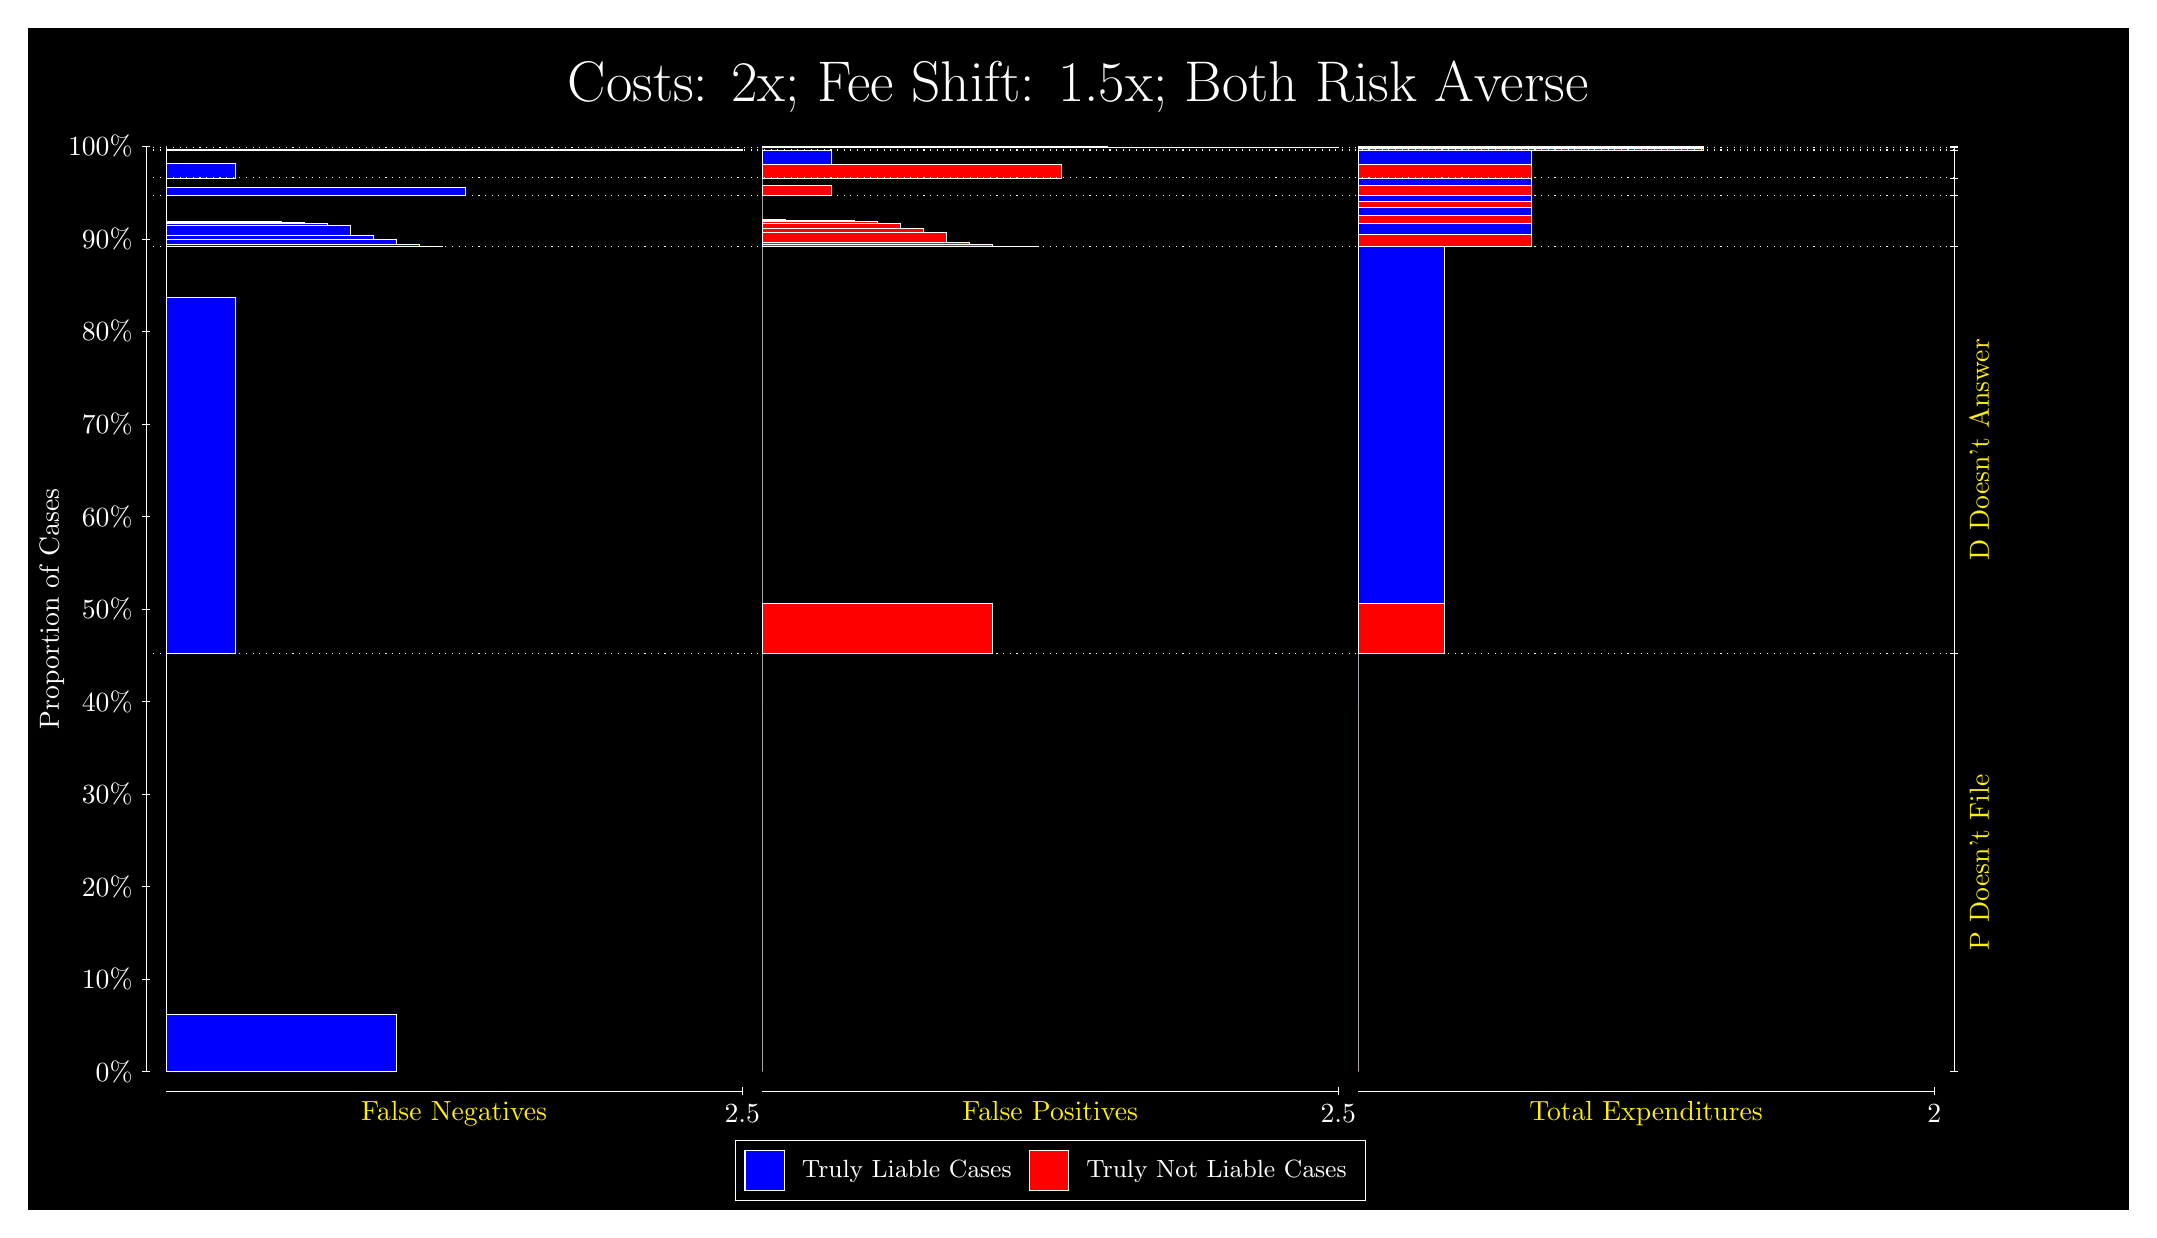
\begin{tikzpicture}
\draw[fill=black] (0,0) rectangle (26.667,15);
\draw[text=white] (0,13.5) rectangle (26.667,15) node[midway] {\huge Costs: 2x; Fee Shift: 1.5x; Both Risk Averse};
\draw[white, very thin] (1.5,1.75) -- (1.5,13.5);
\node[rotate=90, text=white, anchor=center] at (0.3, 7.625) {Proportion of Cases};
\draw[white, very thin] (1.45,1.75) -- (1.55,1.75);
\node[text=white, anchor=east] at (1.45, 1.75) {0\%};
\draw[white, very thin] (1.45,2.925) -- (1.55,2.925);
\node[text=white, anchor=east] at (1.45, 2.925) {10\%};
\draw[white, very thin] (1.45,4.1) -- (1.55,4.1);
\node[text=white, anchor=east] at (1.45, 4.1) {20\%};
\draw[white, very thin] (1.45,5.275) -- (1.55,5.275);
\node[text=white, anchor=east] at (1.45, 5.275) {30\%};
\draw[white, very thin] (1.45,6.45) -- (1.55,6.45);
\node[text=white, anchor=east] at (1.45, 6.45) {40\%};
\draw[white, very thin] (1.45,7.625) -- (1.55,7.625);
\node[text=white, anchor=east] at (1.45, 7.625) {50\%};
\draw[white, very thin] (1.45,8.8) -- (1.55,8.8);
\node[text=white, anchor=east] at (1.45, 8.8) {60\%};
\draw[white, very thin] (1.45,9.975) -- (1.55,9.975);
\node[text=white, anchor=east] at (1.45, 9.975) {70\%};
\draw[white, very thin] (1.45,11.15) -- (1.55,11.15);
\node[text=white, anchor=east] at (1.45, 11.15) {80\%};
\draw[white, very thin] (1.45,12.325) -- (1.55,12.325);
\node[text=white, anchor=east] at (1.45, 12.325) {90\%};
\draw[white, very thin] (1.45,13.5) -- (1.55,13.5);
\node[text=white, anchor=east] at (1.45, 13.5) {100\%};

\draw[white, very thin] (24.457,1.75) -- (24.457,13.5);
\draw[white, very thin] (24.407,1.75) -- (24.507,1.75);
\node[anchor=west] at (24.407, 1.75) {};
\draw[white, very thin] (24.407,7.0616) -- (24.507,7.0616);
\node[anchor=west] at (24.407, 7.0616) {};
\draw[white, very thin] (24.407,12.228) -- (24.507,12.228);
\node[anchor=west] at (24.407, 12.228) {};
\draw[white, very thin] (24.407,12.879) -- (24.507,12.879);
\node[anchor=west] at (24.407, 12.879) {};
\draw[white, very thin] (24.407,13.1) -- (24.507,13.1);
\node[anchor=west] at (24.407, 13.1) {};
\draw[white, very thin] (24.407,13.453) -- (24.507,13.453);
\node[anchor=west] at (24.407, 13.453) {};
\draw[white, very thin] (24.407,13.483) -- (24.507,13.483);
\node[anchor=west] at (24.407, 13.483) {};
\draw[white, very thin] (24.407,13.5) -- (24.507,13.5);
\node[anchor=west] at (24.407, 13.5) {};

\draw[white, very thin, fill=blue] (1.75,1.75) rectangle (4.6775,2.4775);
\draw[white, very thin, fill=red] (1.75,2.4775) rectangle (1.75,7.0616);
\draw[white, very thin, fill=blue] (1.75,7.0616) rectangle (2.6283,11.588);
\draw[white, very thin, fill=red] (1.75,11.588) rectangle (1.75,12.228);
\draw[white, very thin, fill=blue] (1.75,12.228) rectangle (5.2631,12.234);
\draw[white, very thin, fill=blue] (1.75,12.234) rectangle (4.9703,12.254);
\draw[white, very thin, fill=blue] (1.75,12.254) rectangle (4.6775,12.318);
\draw[white, very thin, fill=blue] (1.75,12.318) rectangle (4.3848,12.322);
\draw[white, very thin, fill=blue] (1.75,12.322) rectangle (4.3848,12.372);
\draw[white, very thin, fill=blue] (1.75,12.372) rectangle (4.092,12.499);
\draw[white, very thin, fill=blue] (1.75,12.499) rectangle (3.7993,12.522);
\draw[white, very thin, fill=blue] (1.75,12.522) rectangle (3.5065,12.539);
\draw[white, very thin, fill=blue] (1.75,12.539) rectangle (3.2138,12.542);
\draw[white, very thin, fill=blue] (1.75,12.542) rectangle (2.921,12.547);
\draw[white, very thin, fill=red] (1.75,12.547) rectangle (1.75,12.879);
\draw[white, very thin, fill=blue] (1.75,12.879) rectangle (5.5558,12.979);
\draw[white, very thin, fill=red] (1.75,12.979) rectangle (1.75,13.1);
\draw[white, very thin, fill=blue] (1.75,13.1) rectangle (2.6283,13.284);
\draw[white, very thin, fill=red] (1.75,13.284) rectangle (1.75,13.453);
\draw[white, very thin, fill=blue] (1.75,13.453) rectangle (9.0689,13.463);
\draw[white, very thin, fill=red] (1.75,13.463) rectangle (1.75,13.483);
\draw[white, very thin, fill=red] (1.75,13.483) rectangle (1.75,13.491);
\draw[white, very thin, fill=blue] (1.75,13.491) rectangle (1.75,13.5);
\draw[white, very thin, fill=red] (9.3189,1.75) rectangle (9.3189,6.3341);
\draw[white, very thin, fill=blue] (9.3189,6.3341) rectangle (9.3189,7.0616);
\draw[white, very thin, fill=red] (9.3189,7.0616) rectangle (12.246,7.7015);
\draw[white, very thin, fill=blue] (9.3189,7.7015) rectangle (9.3189,12.228);
\draw[white, very thin, fill=red] (9.3189,12.228) rectangle (12.832,12.232);
\draw[white, very thin, fill=red] (9.3189,12.232) rectangle (12.539,12.236);
\draw[white, very thin, fill=red] (9.3189,12.236) rectangle (12.246,12.254);
\draw[white, very thin, fill=red] (9.3189,12.254) rectangle (11.954,12.279);
\draw[white, very thin, fill=red] (9.3189,12.279) rectangle (11.661,12.407);
\draw[white, very thin, fill=red] (9.3189,12.407) rectangle (11.368,12.462);
\draw[white, very thin, fill=red] (9.3189,12.462) rectangle (11.075,12.529);
\draw[white, very thin, fill=red] (9.3189,12.529) rectangle (10.783,12.551);
\draw[white, very thin, fill=red] (9.3189,12.551) rectangle (10.49,12.561);
\draw[white, very thin, fill=blue] (9.3189,12.561) rectangle (9.9044,12.565);
\draw[white, very thin, fill=blue] (9.3189,12.565) rectangle (9.6116,12.568);
\draw[white, very thin, fill=blue] (9.3189,12.568) rectangle (9.3189,12.879);
\draw[white, very thin, fill=red] (9.3189,12.879) rectangle (10.197,13);
\draw[white, very thin, fill=blue] (9.3189,13) rectangle (9.3189,13.1);
\draw[white, very thin, fill=red] (9.3189,13.1) rectangle (13.125,13.27);
\draw[white, very thin, fill=blue] (9.3189,13.27) rectangle (10.197,13.453);
\draw[white, very thin, fill=red] (9.3189,13.453) rectangle (9.3189,13.474);
\draw[white, very thin, fill=blue] (9.3189,13.474) rectangle (9.3189,13.483);
\draw[white, very thin, fill=red] (9.3189,13.483) rectangle (16.638,13.491);
\draw[white, very thin, fill=blue] (9.3189,13.491) rectangle (13.71,13.5);
\draw[white, very thin, fill=red] (16.888,1.75) rectangle (16.888,6.3341);
\draw[white, very thin, fill=blue] (16.888,6.3341) rectangle (16.888,7.0616);
\draw[white, very thin, fill=red] (16.888,7.0616) rectangle (17.986,7.7015);
\draw[white, very thin, fill=blue] (16.888,7.7015) rectangle (17.986,12.228);
\draw[white, very thin, fill=red] (16.888,12.228) rectangle (19.083,12.378);
\draw[white, very thin, fill=blue] (16.888,12.378) rectangle (19.083,12.524);
\draw[white, very thin, fill=red] (16.888,12.524) rectangle (19.083,12.628);
\draw[white, very thin, fill=blue] (16.888,12.628) rectangle (19.083,12.722);
\draw[white, very thin, fill=red] (16.888,12.722) rectangle (19.083,12.801);
\draw[white, very thin, fill=blue] (16.888,12.801) rectangle (19.083,12.879);
\draw[white, very thin, fill=red] (16.888,12.879) rectangle (19.083,13);
\draw[white, very thin, fill=blue] (16.888,13) rectangle (19.083,13.1);
\draw[white, very thin, fill=red] (16.888,13.1) rectangle (19.083,13.27);
\draw[white, very thin, fill=blue] (16.888,13.27) rectangle (19.083,13.453);
\draw[white, very thin, fill=red] (16.888,13.453) rectangle (21.279,13.474);
\draw[white, very thin, fill=blue] (16.888,13.474) rectangle (21.279,13.483);
\draw[white, very thin, fill=red] (16.888,13.483) rectangle (21.279,13.491);
\draw[white, very thin, fill=blue] (16.888,13.491) rectangle (21.279,13.5);
\draw[white, dotted] (1.5,7.0616) -- (24.457,7.0616);
\draw[white, dotted] (1.5,12.228) -- (24.457,12.228);
\draw[white, dotted] (1.5,12.879) -- (24.457,12.879);
\draw[white, dotted] (1.5,13.1) -- (24.457,13.1);
\draw[white, dotted] (1.5,13.453) -- (24.457,13.453);
\draw[white, dotted] (1.5,13.483) -- (24.457,13.483);
\draw[white, very thin] (1.75,1.5) -- (9.0689,1.5);
\node[text=yellow, anchor=north] at (5.4094, 1.5) {False Negatives};
\draw[white, very thin] (9.0689,1.45) -- (9.0689,1.55);
\node[text=white, anchor=north] at (9.0689, 1.45) {2.5};

\draw[white, very thin] (9.3189,1.5) -- (16.638,1.5);
\node[text=yellow, anchor=north] at (12.978, 1.5) {False Positives};
\draw[white, very thin] (16.638,1.45) -- (16.638,1.55);
\node[text=white, anchor=north] at (16.638, 1.45) {2.5};

\draw[white, very thin] (16.888,1.5) -- (24.207,1.5);
\node[text=yellow, anchor=north] at (20.547, 1.5) {Total Expenditures};
\draw[white, very thin] (24.207,1.45) -- (24.207,1.55);
\node[text=white, anchor=north] at (24.207, 1.45) {2};

\node[text=yellow, centered, rotate=90] at (24.777, 4.4058) {P Doesn't File};
\node[text=yellow, centered, rotate=90] at (24.777, 9.6449) {D Doesn't Answer};






\draw (12.978300999999998,1.5) node[draw=none] (baseCoordinate) {};
\begin{scope}[align=center]
        \matrix[scale=0.5, draw=white, below=0.5cm of baseCoordinate, nodes={draw}, column sep=0.1cm]{
            \node[rectangle, draw, minimum width=0.5cm, minimum height=0.5cm, fill=blue] {}; &
            \node[draw=none, font=\small, text=white] (B) {Truly Liable Cases}; &
            \node[rectangle, draw, minimum width=0.5cm, minimum height=0.5cm, fill=red] {}; &
            \node[draw=none, font=\small, text=white] (B) {Truly Not Liable Cases}; \\
            };
\end{scope}

\end{tikzpicture}
\end{document}